\documentclass[11pt, titlepage]{article}
\usepackage{amsmath,amsthm,amssymb}
\usepackage{hyperref, pgf, tikz}
\usepackage{fancyhdr}
\usetikzlibrary{arrows}
\usepackage[margin=1.25in]{geometry}
\usepackage{graphicx}                     
\pagestyle{fancy}
\usepackage{array}
%\usepackage{wrapfig}

\lhead{Lab \#4}
\rhead{\thepage}
\cfoot{}

\title{Torques, Equilibrium, and Center of Gravity\\ \ \\ \large Lab \#4}
\author{Name: Avery Karlin \\ Partner: Nicholas Yang}
\date{}
\begin{document}

\maketitle

\begin{center}
\LARGE Torques, Equilibrium, and Center of Gravity
\end{center}

\section*{Objective}
The objective of the lab is to measure the spring constant of springs, and the spring constant when they are in series, parallel, and on opposite sides.
\section*{Introduction}

\section*{Procedures and Results}

\begin{figure}[p]
\centering
\hspace*{-10.5cm}
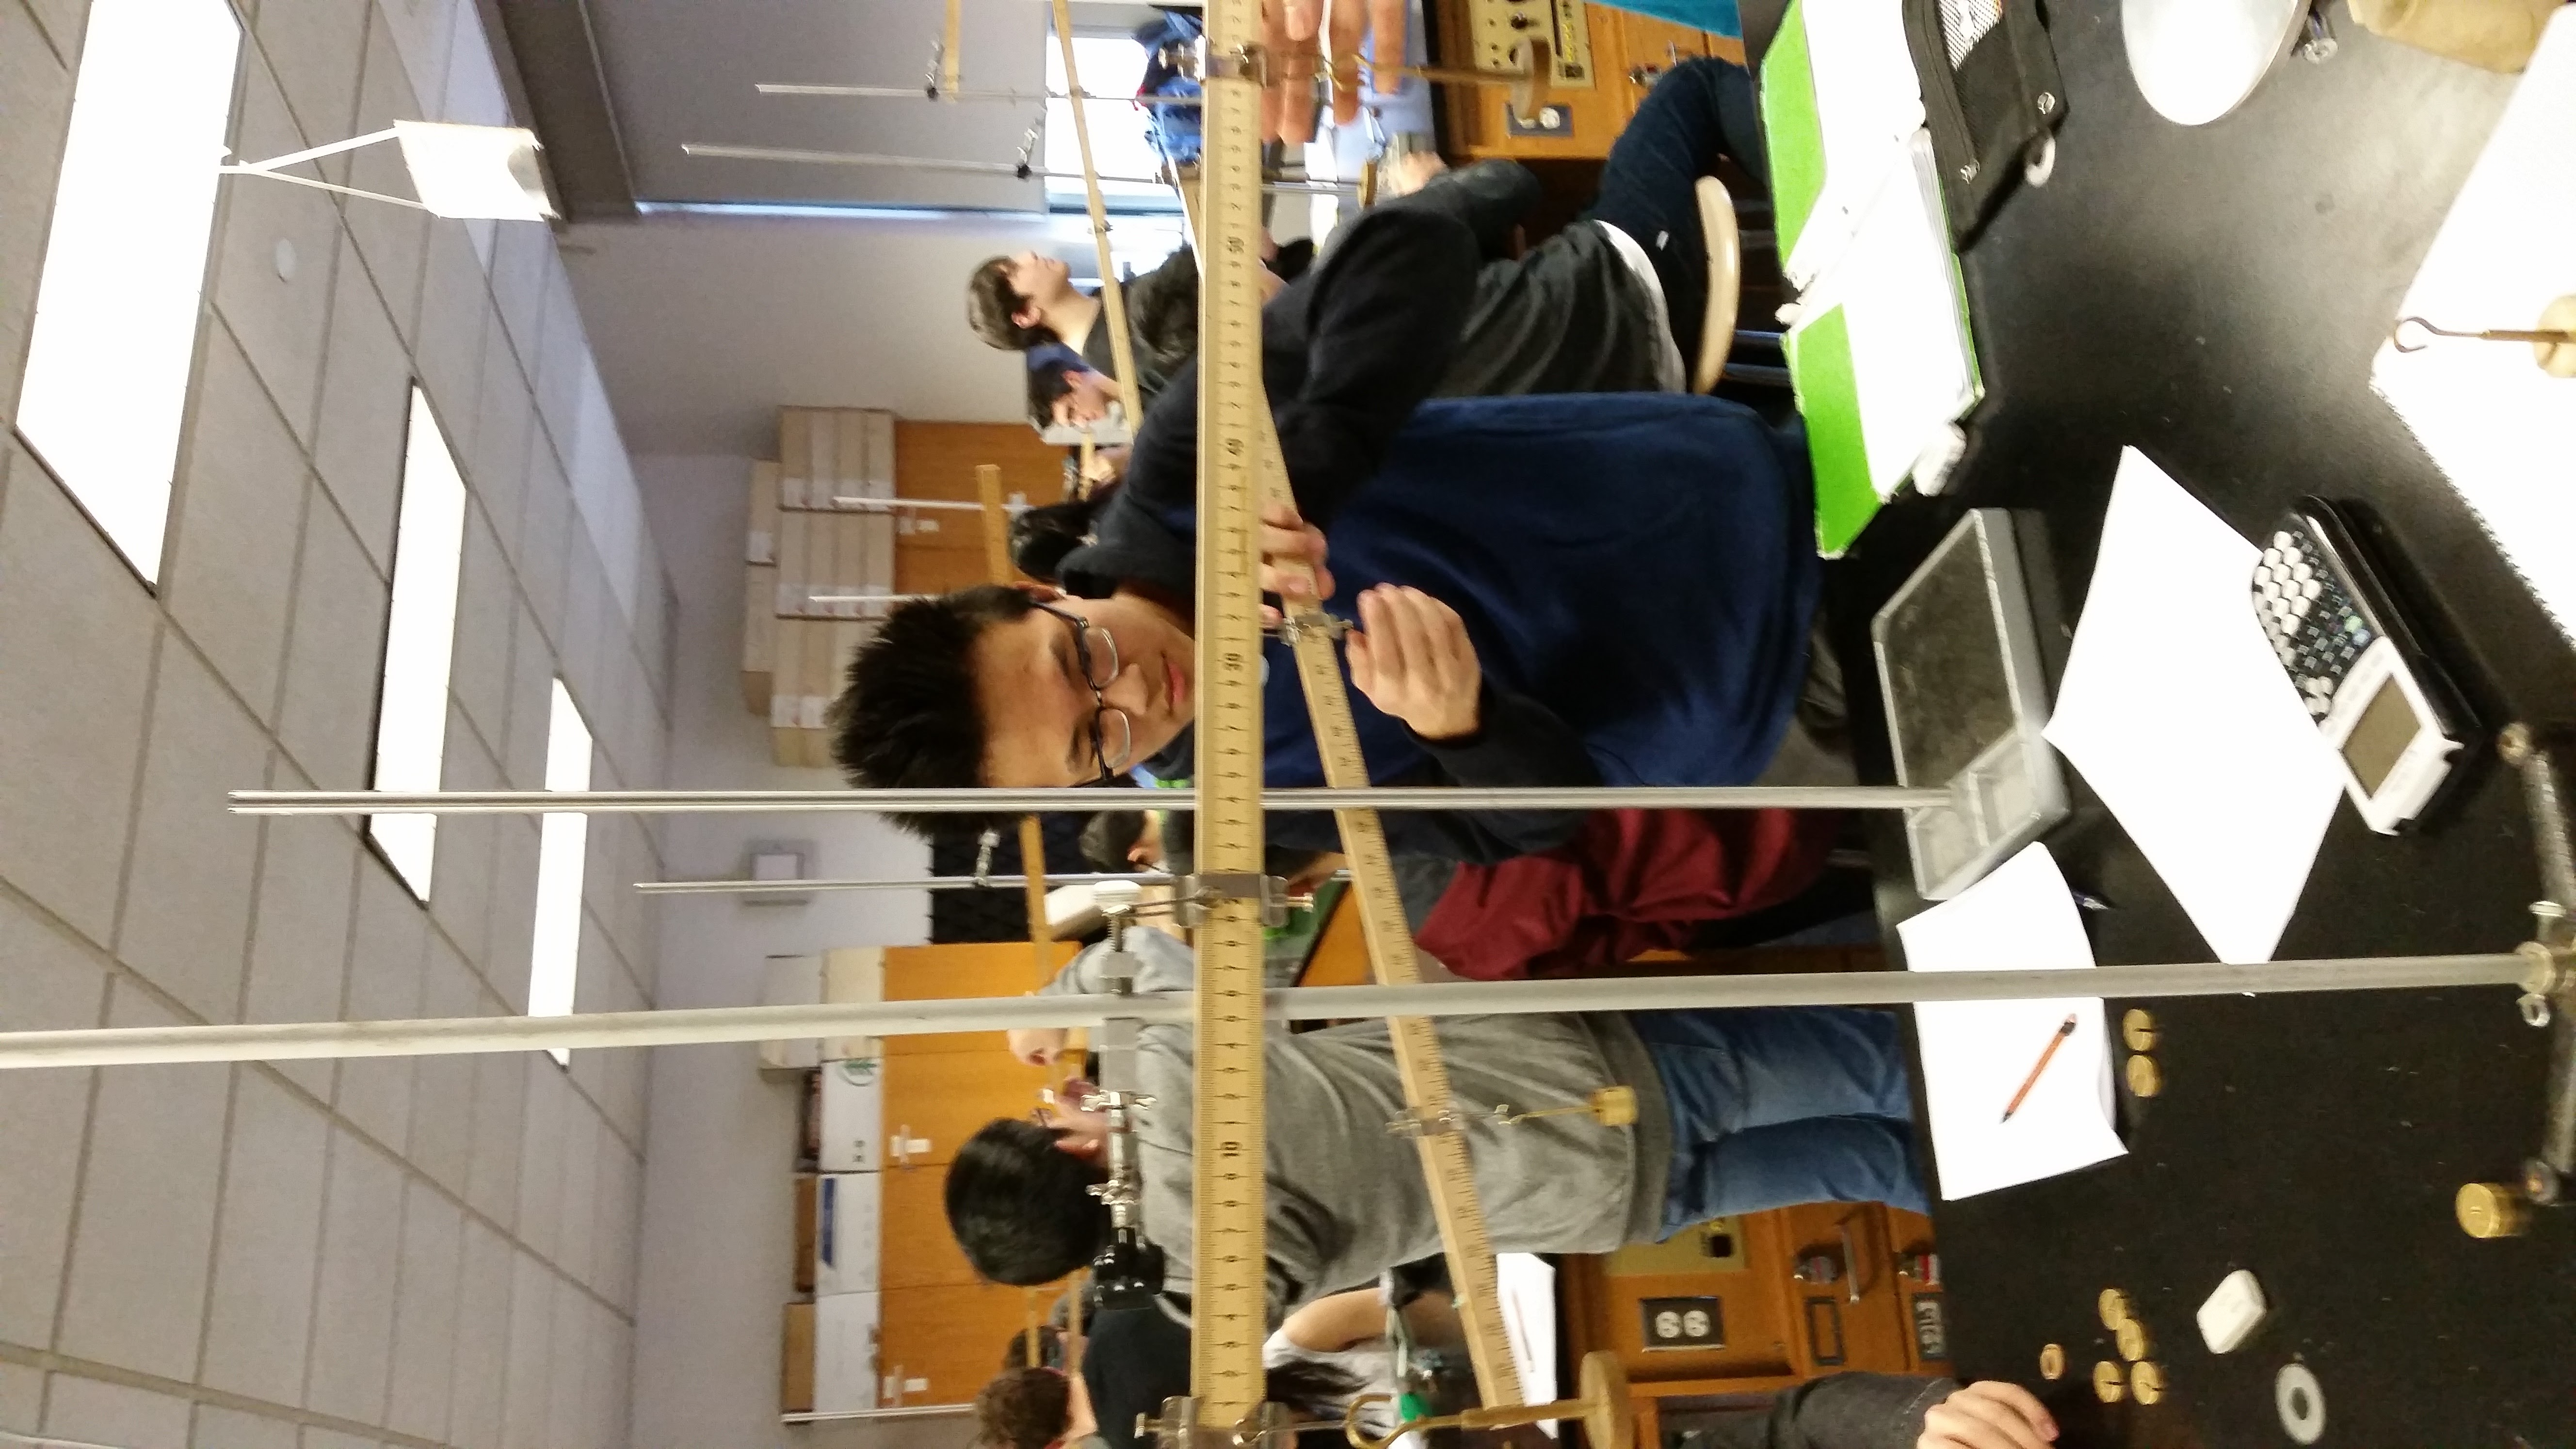
\includegraphics[scale=0.15, angle=270]{lab4.jpg}
\vspace*{19cm}
\end{figure}

\begin{center}
\begin{tabular}
{|m{5em}|m{5em}|m{5em}|m{5em}|m{5em}|m{5em}|}
Spring Format & Trial 1 (s) & 2 & 3 & 4 & 5 \\
Spring \#1 & 3.06 & 2.9 & 3.02 & 2.9 & 2.85 \\
Spring \#2 & 5.8 & 6.08 & 5.8 & 6.05 & 6.08 \\
Series & 6.75 & 6.73 & 6.53 & 6.46 & 6.77 \\
Parallel & 2.56 & 2.88 & 2.68 & 2.6 & 2.88 \\
Opposite & 2.7 & 2.78 & 2.68 & 2.83 & 2.65 \\
\end{tabular}
\end{center}

\section*{Discussion}
Sample calculations for the non-measured data are as shown:

$$\text{Percent Error} = 

\begin{center}
\begin{tabular}
{|m{8em}|m{8em}|m{8em}|m{8em}|}
Spring Format & Average (s) & Period (s) & k (N/m) \\\
Spring \#1 & 2.946 & 1.473 & 9.61 \\
Spring \#2 & 5.922 & 2.961 & 2.377 \\
Series & 6.648 & 3.324 & 1.887 \\
Parallel & 2.72 & 1.36 & 11.27 \\
Opposite & 2.728 & 1.364 & 11.204 \\
\end{tabular}
\end{center}


\section*{Conclusion}


\end{document}
